




\section{Problem Description}

\begin{frame}{Background}
    \begin{itemize}
        \item Distributed Observer Design:
        \item Interconnected System:
        \item Algorithm Proposition:
    \end{itemize}
\end{frame}

\begin{frame}{Interconnected Nonlinear Systems}
    We consider the following interconnected system:
    {\small\begin{equation}
        \begin{aligned}
            \left\{\begin{array}{l}
                     \dot{x}_i= A_{n_i}x_i+B_{n_i}\varphi_i(x_1,\cdots,x_i,u_i) \\
                     y_{i} = C_{n_{i}}x_{i}
                \end{array}\right., \ \forall i \in \mathcal{N},
        \end{aligned}\label{eq:sys}
    \end{equation}}
    where
    {\small\begin{equation*}
        \begin{aligned}
            &A_{n_i}= \begin{bmatrix}
            0_{(n_{i}-1) \times 1} & {I_{(n_{i}-1)}} \\
            0 & 0_{  1 \times (n_{i}-1)}
        \end{bmatrix},\ B_{n_i}= \begin{bmatrix}
            0_{(n_{i}-1)\times1 }, \\ 1
        \end{bmatrix},\\ 
        &
        C_{n_i} = \begin{bmatrix}
            1 & 0_{1 \times (n_{i}-1)}
        \end{bmatrix},
        \end{aligned}
    \end{equation*}}
        with nonlinear function $\varphi_i : \mathbb{R}^{1+\sum^i_{j=1}n_j}\mapsto \mathbb{R}$ satisfying
    {\small\[\big\|\varphi_i\left(x_{[1,i]}+\Delta x_{[1,i]},u_i\right)-\varphi_i\big(x_{[1,i]},u_i\big)\big\|\le L_{\varphi i}\sum^i_{j=1}\sum^{n_i}_{k=1}\big|\Delta x_{j,k}\big|.\]}
    \begin{figure}
        \centering
        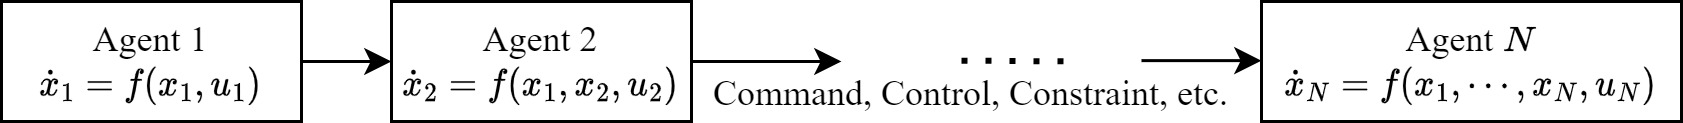
\includegraphics[width=0.8\linewidth]{Fig/Fig_Interconnected_Sys.jpg}
        \caption{Interconnected System in Multi-Agents Systems}
        \label{fig:Interconnected System}
    \end{figure}
\end{frame}

\begin{frame}{Distributed Estimation Scheme}
    \begin{figure}
        \centering
        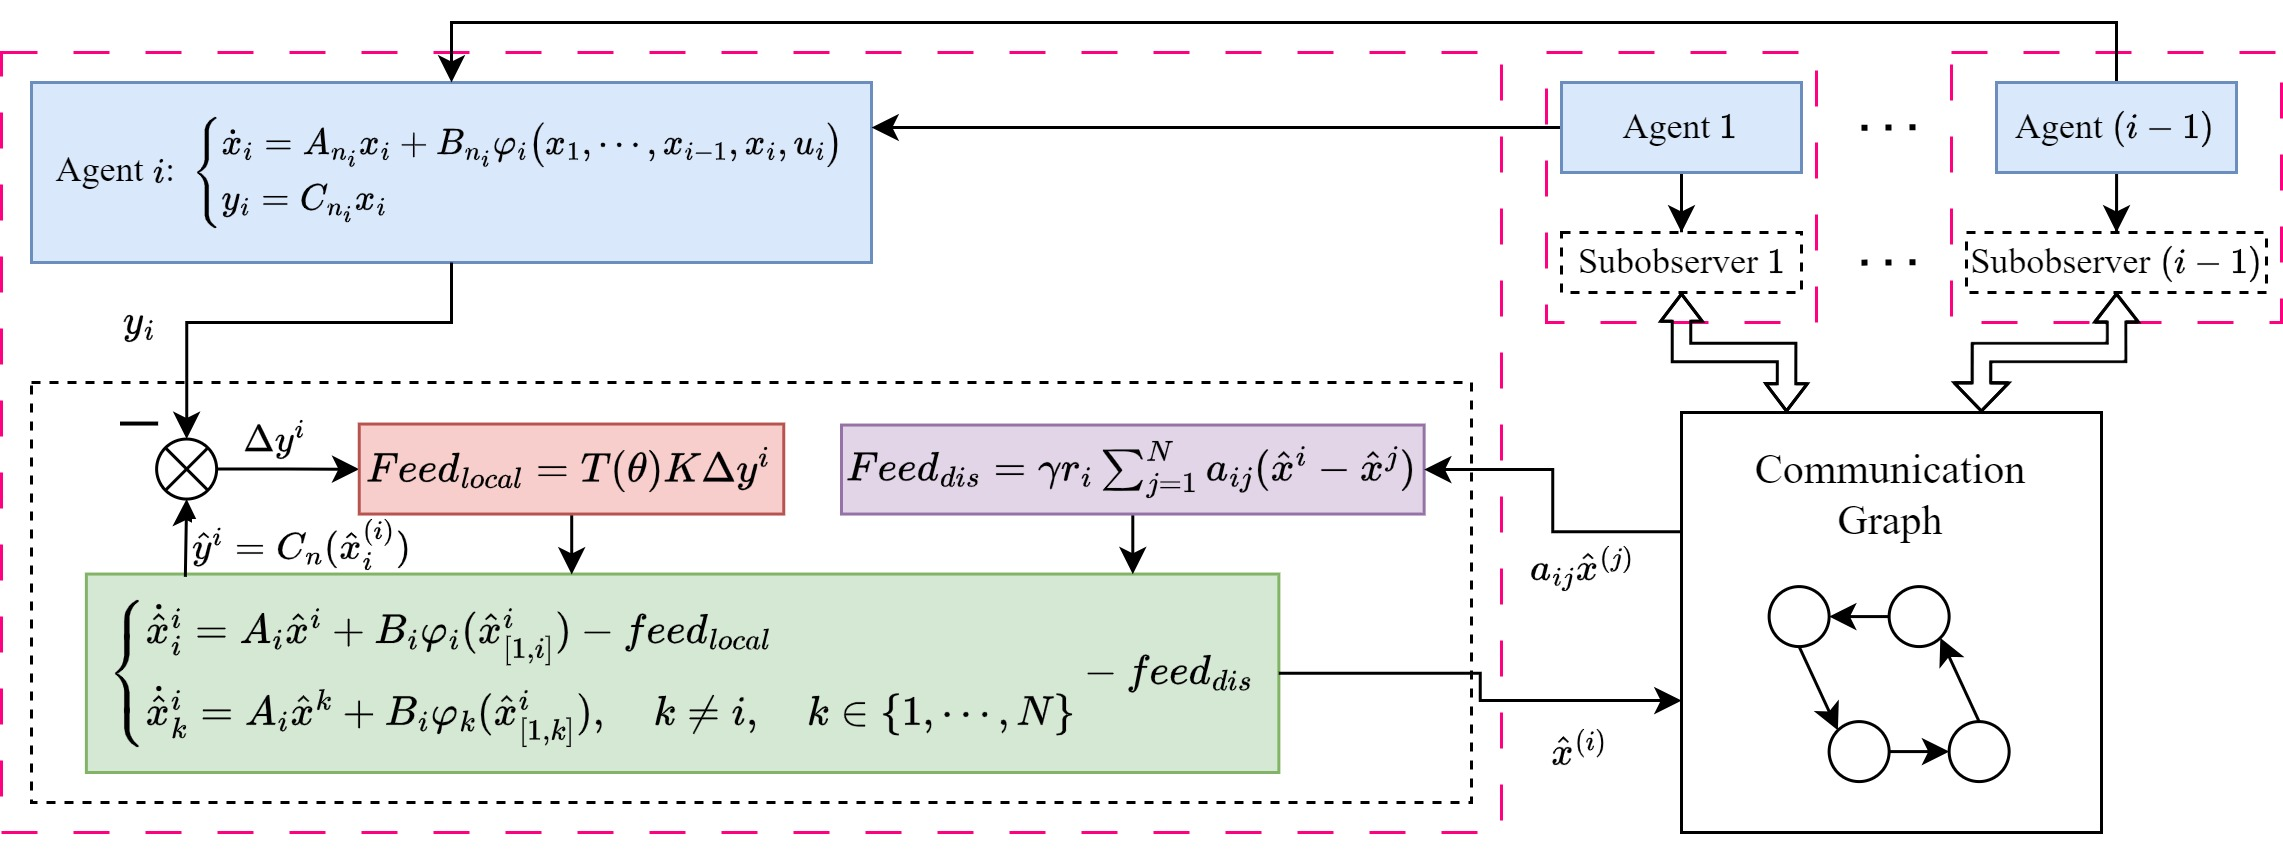
\includegraphics[width=\linewidth]{Fig/Fig_DistributedObserverScheme.jpg}
        \caption{Distributed Observer Scheme for Interconnected System \eqref{eq:sys}}.
        \label{fig:DistributedObserverScheme.png}
    \end{figure}
\end{frame}

\begin{frame}{Distributed High-Gain Observer}
    The local high--gain observer implemented at agent $i$ to estimate the collective state $x$ is given by: 
    \begin{equation}
        \begin{aligned}
            \dot{\hat{x}}^{(i)}=&A\hat{x}^{(i)}+B\varphi(\hat{x}^{(i)},u)+TL_i\big(y_i-C_i \hat{x}^{(i)}\big)\\
            &+\gamma T P_i^{-1}T^{-1}r_i\sum^N_{j=1}a_{ij}\big(\hat{x}^{(j)}-\hat{x}^{(i)}\big),\ i \in \mathcal{N},
        \end{aligned}\label{eq:distributed_HGO}
    \end{equation}
    where $r_i$ is the $i$th entry of the positive row vector $r$.
    The high--gain matrix $T$ is block--diagonal with $T \triangleq \mathrm{diag}(T_1,\cdots, T_N)$, where $T_i\triangleq\mathrm{diag}(\theta_i,\cdots,\theta_i^{n_i})$.
    The feedback matrice, $L_i$ and $P_i$ can be described by 
    \begin{equation}
        \begin{aligned}
            &L_i\triangleq\left[0_{1\times\mathrm{sum}(n_{[1,i-1]})},\ L_{n_i}^\top,\ 0_{1\times\mathrm{sum}(n_{[i+1,N]})}\right]^\top, \\ 
            &P_{i}\triangleq\mathrm{diag}\left(I_{\mathrm{sum}(n_{[1,i-1]})},\ P_{n_{i}},\ I_{\mathrm{sum}(n_{[i+1,N]})}\right).
        \end{aligned}
    \end{equation}
\end{frame}

\begin{frame}{Theory Scheme}
    \begin{figure}
        \centering
        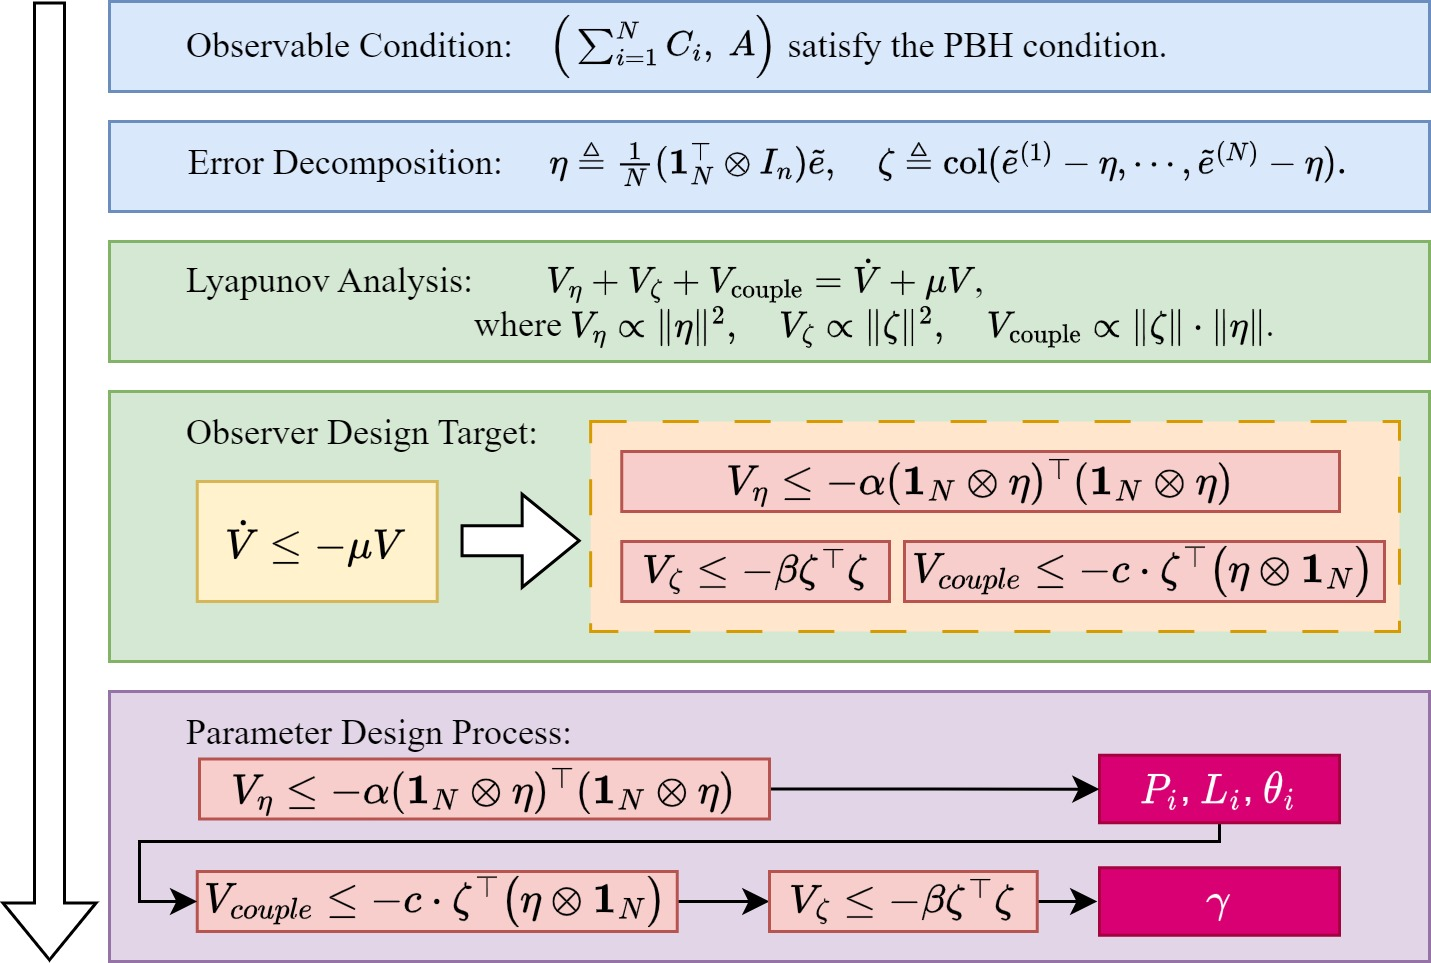
\includegraphics[width=0.7\linewidth]{Fig/Fig_method_diagram.jpg}
        \caption{The main scheme of this work \footnote[frame]{\cite{wu2021design}}}
        \label{fig:Fig_method_diagram}
    \end{figure}
\end{frame}



\section{Error Space Decomposition}
\begin{frame}{Error Decomposition}
    Noticed that in the triangular observable form \eqref{eq:sys}, we have not only the observable pair $\Big(\mathrm{row}(C_1,\cdots,C_N),\ A\Big)$, but also $\Big(\sum^N_{i=1}C_i,\ A\Big)$.

    $\Longrightarrow$ Define the decomposition of the transformed error $\tilde{e}^{(j)}$ of each agent below:
    \[\eta \triangleq \frac{1}{N}\sum^N_{i=1}\tilde{e}^{(k)}_{i}=\frac{1}{N}(\mathbf{1}_N^\top\otimes I_{n})\tilde{e},\quad\zeta\triangleq\mathrm{col}(\tilde{e}^{(1)}-\eta,\ \cdots,\ \tilde{e}^{(N)}-\eta).\]
    
    And the following inequality can be obtained:
    \[\tilde{e}^\top(\hat{\mathcal{L}}\otimes I_n)\tilde{e}=\zeta^\top\Big[\big(U_2\Lambda_{\hat{\mathcal{L}}}U_2^\top\big)\otimes I_n\Big]\zeta\le-\gamma \lambda_2\zeta^\top\zeta, \]
    where $\Lambda_{\hat{\mathcal{L}}}=\mathrm{diag}(m,\lambda_2,\cdots,\lambda_N)$ and $\lambda_i$ follow the same definition in {\it Lemma}~\ref{lemma:laplacian}, and $m$ is a scalar can be randomly chosed since $\sum^N_{i=1}\zeta^{(i)}\equiv0$.
\end{frame}

\begin{frame}{Lyapunov Analysis}
    ??? (The lyapunov decomposition and quadratic forms)
\end{frame}

\begin{frame}{Auxilinary Result}

    \begin{proposition}\footnotesize
        \label{prop:Veta}
            Let the matrices $M_i$ and $M_{ik}$ be the components of $V_\eta$ as defined in (15). If the following matrix inequality holds for all $i \in \{1, \dots, N\}$:
        \begin{equation}
        M_i+N\alpha\cdot I_{n_i} + \sum_{k=1}^{i-1} \big\|M_{ik}\big\| I_{n_i} + \sum_{k=i+1}^{N} \big\|M_{ki}\big\| I_{n_i} \le 0.
        \label{eq:prop eta}
        \end{equation}
        Then the average error component $V_\eta$ is upper bounded by $V_\eta \le -\alpha(\mathbf{1}_N\otimes\eta)^\top(\mathbf{1}_N\otimes\eta)$.    
    \end{proposition}

    \begin{proposition}\footnotesize
        \label{prop:Vzeta}
            Let the matrices $W_i^{(j)}$ and $W_{i,k}^{(j)}$ be the components of $V_\zeta$ as defined in (16). If the following matrix inequality holds for all $i, j \in \mathcal{N}$:
        \begin{equation}
        W_i^{(j)}+\beta I_{n_i} + \sum_{k=1}^{i-1} \big\|W_{ik}^{(j)}\big\| I_{n_i} + \sum_{k=i+1}^{N} \big\|W_{ki}^{(j)}\big\| I_{n_i} \le 0.
        \label{eq:prop zeta}
        \end{equation}
        Then the consensus error component $V_\zeta$ is upper bounded by $V_\zeta \le -\beta\zeta^\top\zeta$.
    \end{proposition}
\end{frame}





\section{Design Algorithm}
\begin{frame}{Main Theorem}

    \begin{theorem}\label{thm:main result}
        \scriptsize
        Consider the MAS~\eqref{eq:sys} and distributed high--gain observer~\eqref{eq:distributed_HGO}. 
        Let the convergence rate $\mu>0$ and $i$th agent's local stability margins $\tau_i>0$ be given. The estimation error $e^{(i)}$ converges exponentially to zero for all $i\in\mathcal{N}$ if there exist symmetric positive definite matrices $P_{n_i}$, full matrices $R_{n_i}$, high--gain parameter $\theta_i>1$ and a consensus gain $\gamma>1$ satifying the following conditions:
        \begin{equation}
            \begin{aligned}
                \mathrm{Sym} \Big( P'_iA_{n_i}  &-R_iC_{n_i}\Big)\le -\tau_iP'_i,
            \end{aligned}\label{eq:condition_DSTDHGO_LMIs}
        \end{equation}
        where $P'_i=(N-1)I_{n_i}+P_{n_i}$.
        The high--gain parameters $\theta_i$ are chosen to satisfy the following inequality for all $i \in \mathcal{N}$:
            \begin{align}
                     \theta_i \ge& \frac{\mu+N+(\sqrt{n_i}+1)L_{\varphi i}}{\tau_i} 
                + \sum_{k=1}^{i-1}\frac{\theta_i^{-n_i}\theta_k^{n_k}\sqrt{n_k}\|P'_{n_i}\|L_{\varphi i}}{\tau_i\lambda_{\min}(P'_{n_i})} + \sum_{k=i+1}^{N}\frac{ \theta_k^{-n_k}\theta_i^{n_i}\sqrt{n_i}\|P'_{n_k}\|L_{\varphi k}}{\tau_i\lambda_{\min}(P'_{n_i})}.
                \label{eq:condition_theta}
            \end{align}
        And the consensus gain $\gamma$ is chosen such that:
            \begin{equation}
                \begin{aligned}
                   \gamma \ge \frac{\beta + Y_{\max}}{\lambda_{2}},
                \end{aligned}\label{eq:condition_gamma}
            \end{equation}
    where $Y_{\max}$ is an upper bound on the coupled error dynamics. The positive scalars $\beta$ and $Y_{\rm max}$ are functions of the system and observer parameters that arise from the Lyapunov proof. Their explicit definitions are provided in Appendix~\ref{appen:def}.
    \end{theorem}

\end{frame}

\begin{frame}{Algorithm}

    {\tiny\begin{algorithm}[H]
        \SetAlgoLined
        \label{alg:observer_design_user}
        \caption{{Observer Design Procedure}}
        \SetKwInOut{KwIn}{Inputs}
        \SetKwInOut{KwOut}{Outputs}
        \KwIn{
            $A_{n_i}$, $C_{n_i}$,$\mathcal{L}$, $r$, $\mu > 0$, $\tau_i > 0$, $L_{\varphi i}$ for $i \in \mathcal{N}$, $\alpha\gg 1$, $c=0$, $Y_{\rm max} =0$\;
        }
        \KwOut{
            $P_{n_i}$, $L_{n_i}$, $\theta_i > 1$, $\gamma > 1$\;
        }
        
        \textbf{\color{blue}Step 1: Calculate feedback matrices:}
        
        \For{$i = 1$ \KwTo $N$}{
            Define $P'_{i} = (N-1)I_{n_i} + P_{n_i}$\;
            Solve the LMI~\eqref{eq:condition_DSTDHGO_LMIs} for $P_{n_i} > 0$ and $R_{n_i}$\;
            {\color{red}$L_{n_i} \leftarrow P^{-1}_{n_i}R_{n_i}$}\;
        }
        
        \textbf{\color{blue}Step 2: Calculate high--gain parameters:}
        
        \For{$i = 1$ \KwTo $N$}{
            \For{$k = 1$ \KwTo $i-1$}{
                $\theta_i \leftarrow \mathrm{max}(1,\text{RHS of \eqref{eq:theta_iteration_extra}})$\;
            }
            $\theta_i \leftarrow \mathrm{max}(1,\text{RHS of \eqref{eq:theta_iteration}})$\;
        }
        
        \textbf{\color{blue}Step 3: Calculate the consensus gain:}
        
        \For{$i = 1$ \KwTo $N$}{
                \For{$k = 1$ \KwTo $i-1$}{
                    $Y_{\max} \leftarrow \text{RHS of \eqref{eq:maxvalue of distributed gain condition}}$\;
                    $c \leftarrow \mathrm{max}(1,\text{RHS of \eqref{eq:max norm of Vcoupling}})$\;
                }
            $\alpha \leftarrow \mathrm{min}\Big(\alpha,\lambda_{\min}\big(P_{n_i}+(N-1)I_{n_i}\big)\Big)$\;
        }
        $\displaystyle\beta \leftarrow \frac{c^2}{\alpha}$; \quad
        $\lambda_2 \leftarrow \mathrm{min}\Big\{\lambda\big(R\mathcal{L}+\mathcal{L}^\top R\big)\Big|\lambda> 0\Big\}$; \quad
        $\displaystyle\gamma \leftarrow \mathrm{max}\Big(1,\ \frac{(\beta + Y_{\max})}{\lambda_{2}}\Big)$.
    \end{algorithm}}


\end{frame}






\section{Simulation Result}
\begin{frame}{Leader Cruising Control (LCC) Based Vehicle Platoon}
    ??? (Model Description)
\end{frame}

\begin{frame}{Simulation Result}
    
\end{frame}






\section{Conclusion}